\chapter{Ondes, modes quantifiés et opérateurs de création}

\section{Ondes, champs et exponentielles complexes}

La théorie quantique des champs est l’outil fondamental de la physique des particules. Avant même de présenter les notions élémentaires d’un champ quantique, il est utile de rassembler les faits mathématiques qui relient les ondes aux particules. Une onde est déjà une configuration de champ : un champ varie d’un point à l’autre de l’espace, et une onde est une configuration dans laquelle ces valeurs oscillent et se propagent. La mécanique quantique établit le lien entre ces ondes et les particules.

La mécanique quantique et la relativité restreinte sont supposées acquises ici. Le but immédiat est de revoir les éléments nécessaires à la physique des particules, et non de remplacer un cours consacré à l’une ou l’autre de ces matières.

Une exponentielle se caractérise par une croissance proportionnelle. Si
\begin{equation}
f(x)=e^{\alpha x},
\end{equation}
alors
\begin{equation}
\frac{df}{dx}=\alpha f.
\end{equation}
Sur un petit intervalle, l’augmentation est proportionnelle à la quantité déjà présente. La croissance d’une population dans une boîte de Petri en donne une image familière : plus il y a d’organismes, plus il y en a qui peuvent se reproduire, de sorte que le taux d’augmentation est proportionnel à la population elle-même. Multiplier \(e^{\alpha x}\) par une constante globale ne change pas cette propriété caractéristique.

Le sinus et le cosinus oscillent au lieu de croître. Ils décrivent la même courbe, décalée d’un quart de période, et la dérivation transforme l’un en l’autre :
\begin{align}
\frac{d}{dx}\sin(kx)&=k\cos(kx),\\
\frac{d}{dx}\cos(kx)&=-k\sin(kx).
\end{align}
Aucune de ces fonctions, prise isolément, n’est une exponentielle, car sa dérivée est proportionnelle à l’autre fonction. En revanche, leur combinaison complexe possède bien la propriété caractéristique d’une exponentielle. Avec \(i^2=-1\),
\begin{align}
\frac{d}{dx}\bigl(\cos(kx)+i\sin(kx)\bigr)
&=-k\sin(kx)+ik\cos(kx)\\
&=ik\bigl(\cos(kx)+i\sin(kx)\bigr).
\end{align}
On a donc
\begin{equation}
e^{ikx}=\cos(kx)+i\sin(kx).
\end{equation}
Cette identité revient sans cesse, car les sinus et les cosinus décrivent des oscillations de type ondulatoire. Lorsque \(x\) est une coordonnée spatiale, la fonction oscille dans l’espace. Lorsque l’argument est le temps, elle oscille au cours du temps.

\section{Fréquence, longueur d’onde et quantité de mouvement du photon}

La fréquence ordinaire \(f\) est le nombre de cycles complets par seconde. Un cycle correspond à une oscillation complète. La fréquence angulaire mesure le même mouvement en radians par seconde :
\begin{equation}
\omega=2\pi f.
\end{equation}
Les deux notations décrivent la même fréquence. On passe de l’une à l’autre pour éviter des facteurs \(2\pi\) inutiles dans un calcul, même si ces facteurs ne disparaissent jamais tout à fait.

La longueur d’onde \(\lambda\) est la distance correspondant à un cycle spatial complet. Si une onde se propage à la vitesse \(v\), le produit de la distance parcourue par cycle et du nombre de cycles par seconde donne la vitesse de propagation :
\begin{equation}
\lambda f=v.
\end{equation}
Pour la lumière dans le vide, \(v=c\), donc
\begin{equation}
\lambda f=c.
\end{equation}
Pour une onde sonore, le membre de droite est la vitesse du son ; pour une onde à la surface de l’eau, c’est la vitesse correspondante. L’apparition de \(c\) est donc une propriété de la lumière, et non une définition valable pour toutes les ondes.

La mécanique quantique fait intervenir la constante de Planck sous deux notations :
\begin{equation}
\hbar=\frac{h}{2\pi}.
\end{equation}
Passer de \(h\) à \(\hbar\) revient simplement à déplacer les facteurs \(2\pi\) d’une équation à l’autre.

Les valeurs numériques des constantes dimensionnées dépendent des unités dans lesquelles on les exprime. Le mètre, la seconde et le kilogramme sont des conventions à l’échelle humaine, pratiques pour les longueurs et les durées ordinaires. Des unités traditionnelles comparables à la longueur d’un bras étaient utiles pour mesurer du tissu ou une corde ; quelle qu’ait été l’histoire précise de la définition du mètre, aucun principe fondamental ne privilégie cette échelle humaine particulière. En unités SI,
\begin{equation}
\begin{aligned}
h &\simeq 6.6\times10^{-34}\ \mathrm{J\,s},
&\hbar &\simeq 1.1\times10^{-34}\ \mathrm{J\,s},\\
c &\simeq 3\times10^8\ \mathrm{m\,s^{-1}}.
\end{aligned}
\end{equation}
Ces nombres donnent une idée des ordres de grandeur dans les unités usuelles : la constante de Planck est extraordinairement petite et la vitesse de la lumière, extraordinairement grande.

Un quantum d’un mode possède une énergie
\begin{equation}
E_{\text{one quantum}}=\hbar\omega=hf.
\end{equation}
C’est l’énergie d’un photon, et non l’énergie totale d’une onde électromagnétique classique quelconque. La fréquence de la lumière visible est de l’ordre de \(10^{15}\) cycles par seconde ; l’énergie typique d’un photon optique est donc de l’ordre de
\begin{equation}
E_\gamma\sim 10^{-19}\ \mathrm{J}.
\end{equation}
Même une oscillation optique aussi rapide correspond à une très faible énergie par quantum, car \(h\) est si petite. Une quantité macroscopique d’énergie optique contient donc un nombre énorme de photons.

L’énergie et la quantité de mouvement méritent une attention particulière, car toutes deux se conservent. Ce sont des grandeurs utiles pour tenir les comptes : l’énergie totale et la quantité de mouvement totale qui entrent dans un processus doivent équilibrer celles qui en sortent. La quantité de mouvement est un vecteur orienté dans le sens du mouvement. Pour une particule qui se déplace beaucoup plus lentement que la lumière,
\begin{equation}
\vec p=m\vec v.
\end{equation}

Considérons maintenant un rayonnement électromagnétique collimaté dans une seule direction, plutôt que dispersé dans plusieurs directions. Sa quantité de mouvement est orientée le long du faisceau. La formule non relativiste ne s’applique pas au photon, car \(m\) désigne la masse au repos, et un photon a une masse au repos nulle. On peut néanmoins se servir d’un aide-mémoire dimensionnel. Si l’on \emph{attribue à tort} au photon la grandeur \(E/c^2\) comme s’il s’agissait d’une masse, puis qu’on substitue \(v=c\), on obtient
\begin{equation}
mv\longrightarrow \frac{E}{c^2}c=\frac{E}{c}.
\end{equation}
Cette manipulation donne par hasard le bon résultat et les bonnes unités, mais elle ne constitue pas un argument valable pour conclure que le photon a une masse au repos \(E/c^2\). La relation relativiste correcte pour un rayonnement collimaté est
\begin{equation}
|\vec p|=\frac{E}{c}.
\end{equation}
L’équation donne la norme. La direction est celle dans laquelle le rayonnement se propage.

Pour un photon,
\begin{align}
|\vec p_\gamma|
&=\frac{E_\gamma}{c}
=\frac{hf}{c}.
\end{align}
Pour la lumière,
\begin{equation}
\lambda f=c,
\qquad
\frac{f}{c}=\frac{1}{\lambda},
\end{equation}
et par conséquent
\begin{equation}
|\vec p_\gamma|=\frac{hf}{c}=\frac{h}{\lambda}.
\end{equation}

\begin{figure}[t]
\centering
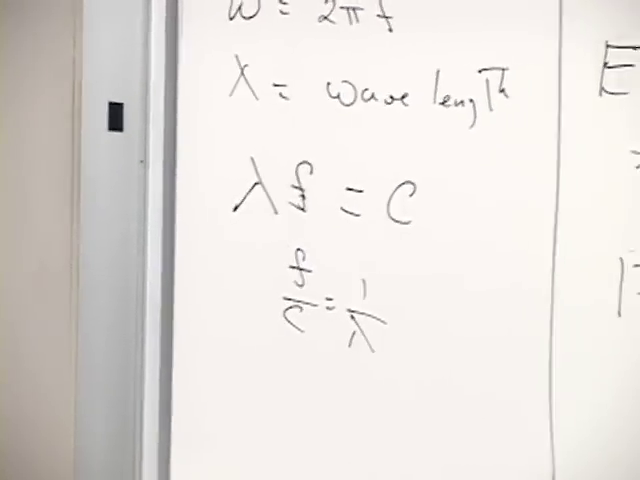
\includegraphics[width=0.56\textwidth]{lecture_02_figure_02.png}
\caption{Pour la lumière, \(\lambda f=c\) et \(f/c=1/\lambda\), les relations utilisées pour obtenir \(|\vec p_\gamma|=h/\lambda\).}
\lectureframe{00:21:39}
\end{figure}

Plus la longueur d’onde est courte, plus la quantité de mouvement du photon est grande. C’est l’un des faits quantiques les plus importants en physique des particules. Pour étudier un objet de petite taille, il faut une sonde de courte longueur d’onde, au prix d’une grande quantité de mouvement.

\begin{classroomqa}
\lecturetimestamp{00:22:23}
\audiencequestion{La relation \(E=\hbar\omega\) est-elle fondamentale, ou découle-t-elle d’un principe plus profond ?}
\lecturerresponse{Elle découle de la mécanique quantique de l’oscillateur harmonique. Nous utiliserons ce résultat ici sans en reprendre la démonstration ; la description par l’oscillateur développée ci-dessous en donnera le cadre plus profond.}
\end{classroomqa}


\section{Amplitude d’une onde et nombre de photons}

\begin{classroomqa}
\lecturetimestamp{00:23:10}
\audiencequestion{Que signifie l’amplitude d’une onde en termes de photons ?}
\lecturerresponse{Comparons deux ondes de même longueur d’onde et de même fréquence, mais d’amplitudes différentes, par exemple \(\sin(kx)\) et \(A\sin(kx)\). En physique classique, l’énergie contenue dans une région donnée est proportionnelle au carré de l’amplitude. En mécanique quantique, un mode qui contient \(n\) photons possède une énergie \(n\hbar\omega\). À fréquence, région et normalisation fixées, l’ordre de grandeur de l’amplitude croît donc comme \(\sqrt n\).}
\end{classroomqa}

Les deux ondes ont le même profil d’oscillation. L’une est simplement plus intense que l’autre.\footnote{Le schéma reprend la comparaison des ondes à 00:23:47--00:24:28.}

\begin{figure}[t]
\centering
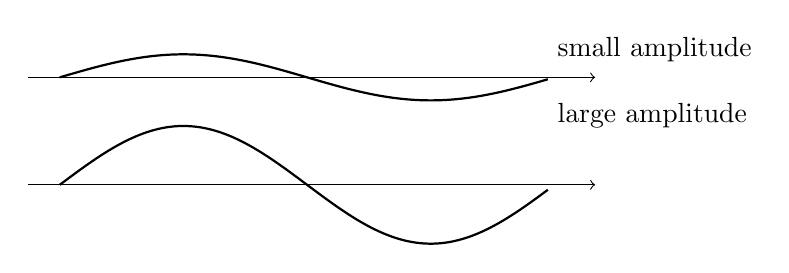
\begin{tikzpicture}[x=1cm,y=0.65cm]
\draw[->] (-0.4,0) -- (6.8,0);
\draw[->] (-0.4,-2.1) -- (6.8,-2.1);
\draw[thick] plot[domain=0:6.2,samples=120] (\x,{0.45*sin(\x r)});
\draw[thick] plot[domain=0:6.2,samples=120] (\x,{-2.1+1.15*sin(\x r)});
\draw (6.2,0.55) node[right]{small amplitude};
\draw (6.2,-0.75) node[right]{large amplitude};
\end{tikzpicture}
\caption{Ondes de même longueur d’onde et de même fréquence, mais d’amplitudes différentes.}
\end{figure}

Pour une quantité d’onde fixée,
\begin{equation}
E_{\text{wave}}\propto A^2.
\end{equation}
Pour une onde électromagnétique, cela correspond à l’affirmation bien connue selon laquelle l’énergie du champ est proportionnelle au carré de son intensité. Si le même mode contient \(n\) photons, alors
\begin{equation}
E_{\text{wave}}=n\hbar\omega.
\end{equation}
Par conséquent, si le mode, la fréquence, la normalisation et la région sont fixés,
\begin{equation}
A^2\propto n\hbar\omega,
\qquad
A\propto\sqrt n\quad\text{at fixed }\omega.
\end{equation}
Il ne s’agit pas d’affirmer une normalisation exacte. La quantité d’onde considérée compte : doubler la longueur d’une onde par ailleurs uniforme modifie son énergie totale sans changer l’amplitude locale. On peut donc comprendre cette proportionnalité pour une région fixée, par exemple une longueur d’onde.

Il faut aussi apporter une précision propre à la mécanique quantique. L’amplitude et la phase ne peuvent pas toutes deux recevoir des valeurs classiques exactes. La question ``Quelle est l’amplitude d’un photon ?''est donc ambiguë si elle demande un champ classique parfaitement défini. Poser \(n=1\) fournit néanmoins une échelle d’ordre de grandeur pertinente.

\begin{classroomqa}
\lecturetimestamp{00:28:25}
\audiencequestion{Dans un schéma d’onde électromagnétique, le déplacement vertical représente-t-il la position spatiale du photon ?}
\lecturerresponse{Non. L’axe de propagation est spatial, tandis que la coordonnée verticale représente la valeur du champ électrique ou magnétique. La quantité de mouvement est orientée le long de l’axe de propagation, et non dans la direction de l’amplitude du champ représentée sur le graphique.}
\end{classroomqa}

L’onde peut se propager dans n’importe quelle direction de l’espace, mais le schéma sinusoïdal habituel n’utilise son axe horizontal que comme coordonnée spatiale. L’autre axe représente l’intensité du champ.

\begin{classroomqa}
\lecturetimestamp{00:29:37}
\audiencequestion{Le nombre de photons indiqué est-il compté sur une longueur d’onde ou une période de l’onde ?}
\lecturerresponse{On peut choisir une région fixée, par exemple une longueur d’onde. C’est pourquoi la relation n’est qu’une proportionnalité : l’énergie totale et le nombre de photons dépendent aussi de la quantité d’onde considérée. À amplitude identique, deux, trois ou quatre longueurs d’onde contiennent respectivement plus d’énergie qu’une seule.}
\end{classroomqa}

\begin{classroomqa}
\lecturetimestamp{00:30:17}
\audiencequestion{L’amplitude d’un photon unique n’a-t-elle aucun sens ?}
\lecturerresponse{Elle n’a de sens que comme indication d’ordre de grandeur, obtenue en posant \(n=1\). Pour un mode électromagnétique, les informations sur les champs électrique et magnétique jouent un rôle analogue à celui des informations sur la position et la quantité de mouvement conjuguées ; l’incertitude quantique limite donc la précision avec laquelle on peut attribuer une amplitude classique. La relation d’ordre de grandeur reste utile.}
\end{classroomqa}

Ces questions nous amènent déjà à la théorie quantique des champs, où le lien entre les variables de champ et le nombre de particules peut être formulé avec précision. Pour l’instant, les relations de proportionnalité suffisent.

\section{Relations quantiques générales et ondes de matière lentes}

Certaines formules introduites pour les photons s’appliquent à des situations beaucoup plus générales, tandis que d’autres ne le font pas. Il est utile de faire le point avant de passer aux électrons.

\begin{figure}[t]
\centering
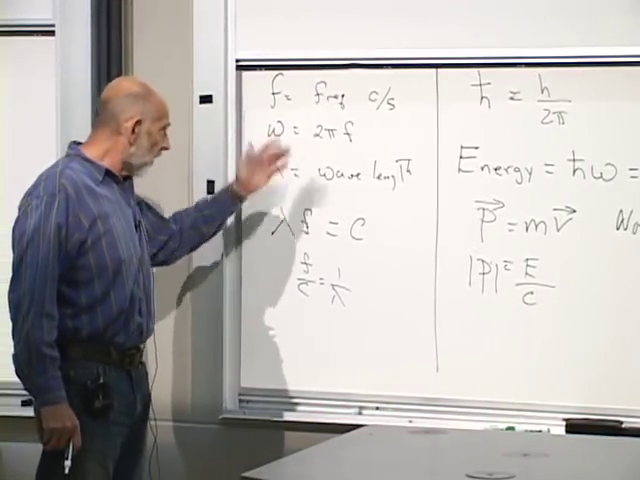
\includegraphics[width=0.82\textwidth]{lecture_02_figure_03.png}
\caption{Définitions des ondes et relations de quantité de mouvement pour les photons et pour le régime non relativiste, avec leurs domaines de validité.}
\lectureframe{00:31:52}
\end{figure}

Les définitions de \(f\), \(\omega=2\pi f\) et \(\lambda\) s’appliquent de façon générale. La relation quantique
\begin{equation}
E=\hbar\omega=hf
\end{equation}
est également générale dans le cadre de cette discussion. En revanche, les formules qui contiennent \(c\), comme \(\lambda f=c\) et \(|\vec p|=E/c\), s’appliquent aux ondes qui se déplacent à la vitesse de la lumière. La formule \(\vec p=m\vec v\) s’applique aux particules qui se déplacent beaucoup plus lentement que la lumière. Le mouvement relativiste entre ces deux régimes requiert une interpolation dont nous n’avons pas encore besoin.

La relation quantité de mouvement--longueur d’onde subsiste après l’exemple du photon :
\begin{equation}
p=\frac{h}{\lambda}.
\end{equation}
Ici, \(p\) désigne la norme lorsque \(\lambda\) est prise comme une longueur d’onde positive ; on peut préciser la direction séparément.

\begin{figure}[t]
\centering
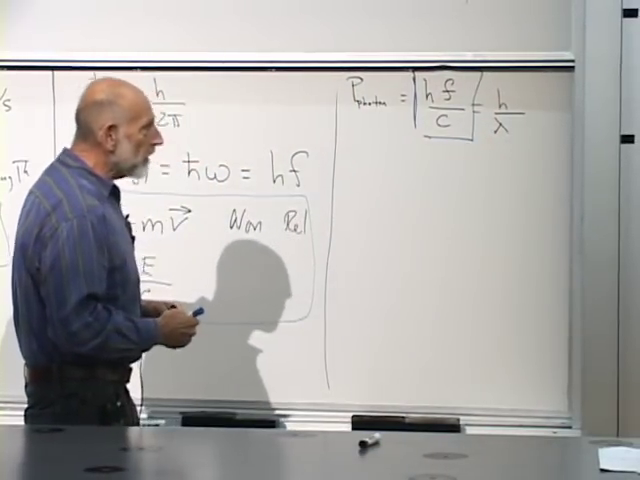
\includegraphics[width=0.74\textwidth]{lecture_02_figure_04.png}
\caption{Quantité de mouvement du photon \(|\vec p_\gamma|=hf/c=h/\lambda\), qui conduit à la relation générale de de Broglie.}
\lectureframe{00:33:32}
\end{figure}

On peut associer une onde à un électron, à un noyau, et même à une boule de bowling. Les interférences électroniques en sont une manifestation. Écrivons l’onde électronique sous la forme \(\psi\). Quelle relation remplace \(\lambda f=c\) pour un électron se déplaçant lentement ? Il nous manque la relation non relativiste entre l’énergie et la quantité de mouvement.

Partons de l’énergie cinétique et de la quantité de mouvement :
\begin{align}
E&=\frac12 mv^2,\\
p&=mv,
\qquad
v=\frac{p}{m}.
\end{align}
En substituant la dernière relation dans la première, on obtient
\begin{align}
E
&=\frac12m\left(\frac{p}{m}\right)^2\\
&=\frac{p^2}{2m}.
\end{align}
La masse apparaît au numérateur dans \(\frac12 mv^2\) et au dénominateur dans \(p^2/(2m)\). Cette disposition est facile à confondre et utile à retrouver par le calcul.

Utilisons maintenant les relations quantiques générales
\begin{equation}
E=hf,
\qquad
p=\frac{h}{\lambda}.
\end{equation}
Pour une particule unique lente,
\begin{align}
hf
&=\frac{p^2}{2m}\\
&=\frac{1}{2m}\left(\frac{h}{\lambda}\right)^2\\
&=\frac{h^2}{2m\lambda^2}.
\end{align}
En divisant par \(h\), on obtient
\begin{equation}
f=\frac{h}{2m\lambda^2}.
\end{equation}

\begin{figure}[t]
\centering
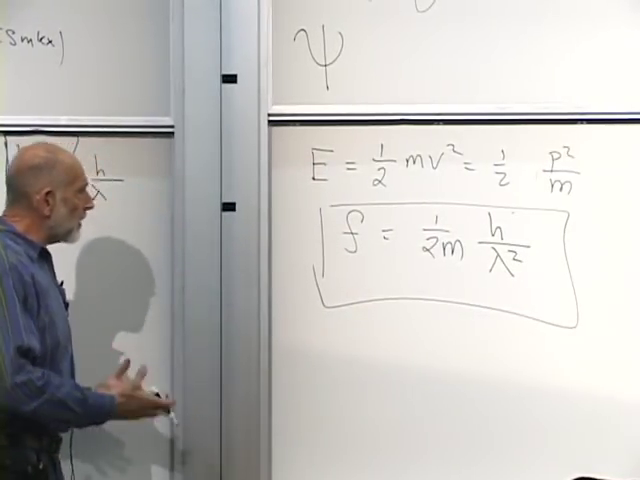
\includegraphics[width=0.64\textwidth]{lecture_02_figure_05.png}
\caption{Pour une particule lente, \(E=p^2/(2m)\) et \(p=h/\lambda\) donnent \(f=h/(2m\lambda^2)\).}
\lectureframe{00:37:47}
\end{figure}

Pour la lumière,
\begin{equation}
f\propto\frac{1}{\lambda},
\end{equation}
alors que, pour une matière lente,
\begin{equation}
f\propto\frac{1}{\lambda^2}.
\end{equation}
Il n’est pas nécessaire de mémoriser isolément la seconde relation. On peut toujours la retrouver à partir de \(E=p^2/(2m)\), \(E=hf\) et \(p=h/\lambda\). Pour un électron qui se déplace lentement dans un atome, elle donne la fréquence de l’onde de Schr\"odinger correspondante.

\begin{classroomqa}
\lecturetimestamp{00:38:35}
\audiencequestion{La relation non relativiste fréquence--longueur d’onde s’applique-t-elle à d’autres particules que les électrons ?}
\lecturerresponse{Oui. Elle s’applique à toute particule qui se déplace beaucoup plus lentement que la lumière. L’interpolation relativiste entre les régimes lent et lumineux constitue un sujet distinct.}
\end{classroomqa}

\begin{classroomqa}
\lecturetimestamp{00:38:55}
\audiencequestion{Quelle relation s’applique à un neutrino ?}
\lecturerresponse{Cela dépend de la vitesse du neutrino. La plupart des neutrinos rencontrés dans la nature se déplacent très près de la vitesse de la lumière, si bien que la relation du régime lumineux constitue une bonne approximation. Un neutrino qui se déplacerait beaucoup plus lentement que la lumière obéirait plutôt à la relation non relativiste.}
\end{classroomqa}

\editorialnote{Un bref échange avec le public, immédiatement après la question sur les neutrinos, porte sur les amplitudes, les quanta et les différentes longueurs d’onde des électrons, mais sa formulation est trop altérée pour être restituée avec certitude. La réponse que l’on peut reconstituer reporte à plus tard la relation générale entre les amplitudes et les quanta de longueurs d’onde différentes.}

\begin{classroomqa}
\lecturetimestamp{00:39:56}
\audiencequestion{Un électron provenant d’un accélérateur de \(20\,\mathrm{keV}\) est-il lent ou relativiste ?}
\lecturerresponse{On le traite comme une particule lente. Dans un système d’unités où \(c=1\), la masse, l’énergie et la quantité de mouvement peuvent s’exprimer dans les mêmes unités. L’échelle de l’énergie de masse au repos de l’électron est d’environ \(0.5\,\mathrm{MeV}\), tandis que \(20\,\mathrm{keV}\) est beaucoup plus petit. De manière équivalente, le critère non relativiste sur la quantité de mouvement est \(p\ll mc\).}
\end{classroomqa}

La comparaison des énergies dans cet exemple est
\begin{equation}
K=20\,\mathrm{keV}\ll m_ec^2\simeq0.5\,\mathrm{MeV}.
\end{equation}
\editorialnote{Dans le passage source à 00:39:56--00:41:40, \(20\,\mathrm{keV}\) est présenté comme l’énergie d’un accélérateur, puis le critère relativiste est formulé en comparant la quantité de mouvement à la masse au repos. Énoncer séparément les critères sur l’énergie cinétique et sur la quantité de mouvement évite d’assimiler l’énergie indiquée à une quantité de mouvement, tout en conservant la conclusion selon laquelle le régime est non relativiste.}

\section{Vitesse de phase, vitesse de groupe et dispersion}

\begin{classroomqa}
\lecturetimestamp{00:41:46}
\audiencequestion{Peut-on obtenir la vitesse d’une onde électronique en multipliant sa fréquence par sa longueur d’onde ?}
\lecturerresponse{On obtient la vitesse de phase, et non la vitesse attribuée à l’électron. Un paquet localisé possède à la fois une vitesse de phase, qui décrit le mouvement de ses crêtes et de ses creux internes, et une vitesse de groupe, qui décrit le mouvement de l’enveloppe. C’est la vitesse de groupe qui est identifiée au mouvement de la particule.}
\end{classroomqa}

Un paquet d’ondes ressemble localement à un sinus ou à un cosinus, mais il est délimité par une enveloppe. En se propageant, l’enveloppe et les crêtes qu’elle contient ne sont pas nécessairement animées de la même vitesse.\footnote{Le schéma reprend la discussion du paquet d’ondes à 00:42:34--00:44:11.}

\begin{figure}[t]
\centering
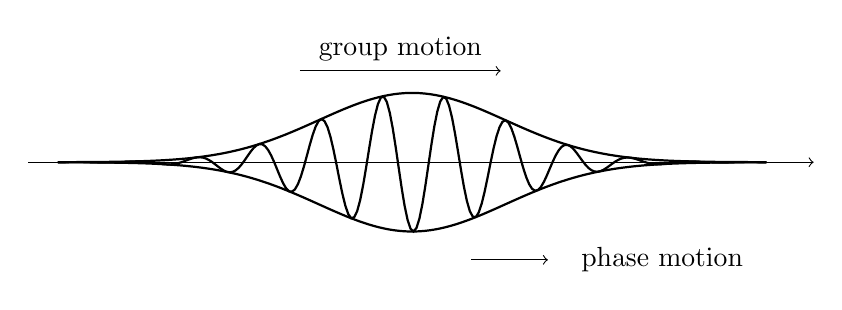
\begin{tikzpicture}[x=0.75cm,y=0.8cm]
\draw[->] (-0.5,0) -- (12.8,0);
\draw[thick] plot[domain=0:12,samples=140] (\x,{1.10*exp(-0.20*(\x-6)^2)});
\draw[thick] plot[domain=0:12,samples=140] (\x,{-1.10*exp(-0.20*(\x-6)^2)});
\draw[thick] plot[domain=0:12,samples=240] (\x,{1.10*exp(-0.20*(\x-6)^2)*sin(6*\x r)});
\draw[->] (4.1,1.45) -- (7.5,1.45);
\draw (5.8,1.8) node{group motion};
\draw[->] (7.0,-1.55) -- (8.3,-1.55);
\draw (8.7,-1.55) node[right]{phase motion};
\end{tikzpicture}
\caption{Paquet d’ondes localisé dont l’enveloppe et la phase interne se propagent généralement à des vitesses différentes.}
\end{figure}

La vitesse de phase est celle des crêtes, des creux et des autres phases fixes d’une composante monochromatique. Pour la relation de dispersion non relativiste,
\begin{equation}
v_\phi=f\lambda=\frac{h}{2m\lambda}.
\end{equation}
Elle dépend de la longueur d’onde. Les différentes composantes de longueur d’onde ont donc des vitesses de phase différentes ; les crêtes peuvent ainsi défiler dans le paquet, qui peut alors se disperser. La vitesse de groupe est celle du paquet dans son ensemble, et c’est elle que l’on identifie à la particule.

Il existe un cas particulier simple. Si toutes les composantes de longueur d’onde se propagent à la même vitesse, les vitesses de phase et de groupe coïncident. La lumière dans le vide possède cette propriété : toutes les longueurs d’onde se propagent à \(c\). Ce n’est pas le cas de la relation pour les particules lentes : \(f\lambda\) varie avec \(\lambda\).

L’équation
\begin{equation}
f=\frac{h}{2m\lambda^2}
\end{equation}
est l’équation libre de Schr\"odinger sous une forme légèrement déguisée. La fréquence détermine la dépendance temporelle d’une onde plane, la longueur d’onde en détermine la dépendance spatiale, et l’équation de Schr\"odinger relie les deux. Réciproquement, substituer une onde de fréquence et de longueur d’onde déterminées dans l’équation libre de Schr\"odinger redonne cette relation de dispersion.

\begin{classroomqa}
\lecturetimestamp{00:47:02}
\audiencequestion{La vitesse de phase peut-elle dépasser celle de la lumière ?}
\lecturerresponse{Oui. La vitesse de phase ne transporte pas d’information. L’information et le paquet localisé se propagent à la vitesse de groupe ; une vitesse de phase supraluminique ne permet donc pas de transmettre un signal plus vite que la lumière.}
\end{classroomqa}

\section{Espace fini et quantité de mouvement discrète}

Nous nous intéresserons finalement aux ondes dans un espace infini, mais il est plus sûr de commencer par un système fini. Un ordinateur ne peut ni stocker ni manipuler directement l’infini. On formule d’abord les équations pour un système fini, puis on prend la limite où sa taille devient arbitrairement grande. Cette méthode est utile dans toute la mécanique quantique, la théorie quantique des champs et la physique des particules.

Commencer en une dimension spatiale ne fait perdre rien d’essentiel. L’onde peut se propager sur une corde de violon, sur une corde que l’on agite ou dans un monde abstrait à une dimension. Le système fini le plus évident est un segment de longueur \(L\) dont les extrémités réfléchissent l’onde. Celle-ci atteint une extrémité, se réfléchit et repart en sens inverse. Cette condition aux limites réfléchissante est tout à fait légitime, mais elle présente un inconvénient : la quantité de mouvement n’est pas conservée dans le système ondulatoire. Une onde qui se propage vers la droite porte une quantité de mouvement orientée vers la droite ; après réflexion, celle-ci est orientée vers la gauche. La limite a fourni l’impulsion et absorbé la différence.

L’inversion de la quantité de mouvement à une extrémité réfléchissante peut être représentée schématiquement.\footnote{Le schéma reprend l’argument sur la limite réfléchissante à 00:49:24--00:51:08.}

\begin{figure}[t]
\centering
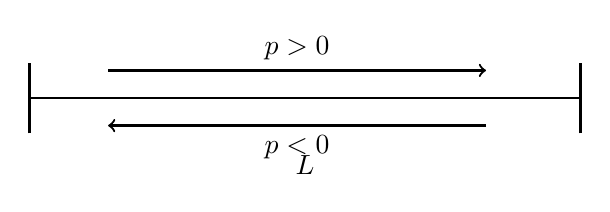
\begin{tikzpicture}[x=1cm,y=1cm]
\draw[thick] (0,0) -- (7,0);
\draw[very thick] (0,-0.45) -- (0,0.45);
\draw[very thick] (7,-0.45) -- (7,0.45);
\draw[->,thick] (1.0,0.35) -- (5.8,0.35) node[midway,above]{\(p>0\)};
\draw[->,thick] (5.8,-0.35) -- (1.0,-0.35) node[midway,below]{\(p<0\)};
\draw (3.5,-0.85) node{\(L\)};
\end{tikzpicture}
\caption{La réflexion aux extrémités d’un segment fini inverse la quantité de mouvement d’une onde en propagation.}
\end{figure}

Il existe une autre façon de rendre le système fini tout en conservant la quantité de mouvement : identifier les deux extrémités du segment. On peut représenter le résultat comme un cercle, mais il n’est pas nécessaire d’imaginer un cercle réel plongé dans une deuxième dimension. La formulation mathématique se réduit à dire que la coordonnée est périodique : après avoir parcouru une distance totale \(L\), on revient au même point.

\begin{figure}[t]
\centering
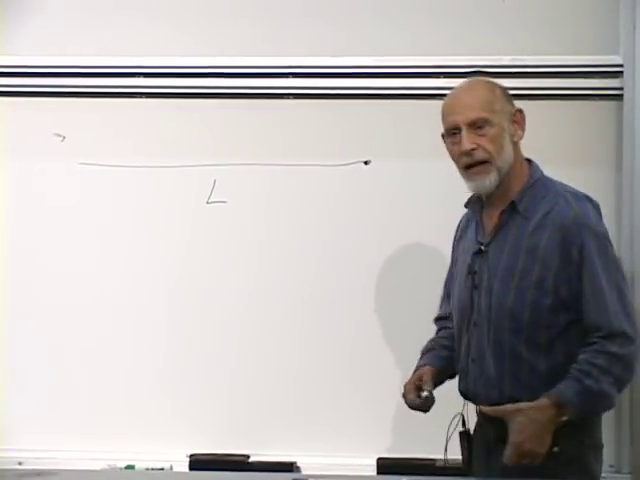
\includegraphics[width=0.72\textwidth]{lecture_02_figure_06.png}
\caption{Trajet unidimensionnel de longueur totale \(L\), servant à introduire l’identification périodique.}
\lectureframe{00:51:21}
\end{figure}

L’identification des extrémités est illustrée explicitement dans le schéma suivant.\footnote{Le schéma reprend l’argument sur l’identification périodique à 00:51:09--00:52:37.}

\begin{figure}[t]
\centering
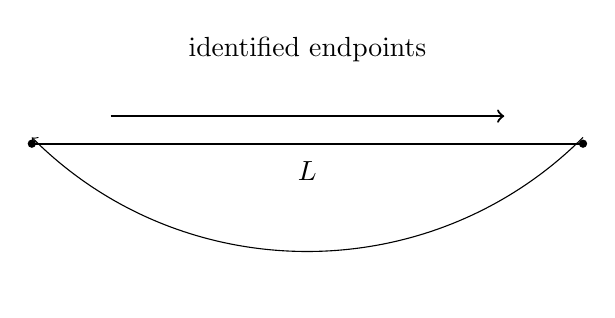
\begin{tikzpicture}[x=1cm,y=1cm]
\draw[thick] (0,0) -- (7,0);
\fill (0,0) circle (1.5pt);
\fill (7,0) circle (1.5pt);
\draw[->,thick] (1.0,0.35) -- (6.0,0.35);
\draw (3.5,-0.35) node{\(L\)};
\draw[->,bend left=45] (7,0.08) to (0,0.08);
\draw (3.5,1.2) node{identified endpoints};
\end{tikzpicture}
\caption{Espace unidimensionnel périodique obtenu en identifiant les extrémités d’un trajet de longueur \(L\).}
\end{figure}

Une onde qui se déplace vers la droite atteint alors l’extrémité représentée, réapparaît au début du trajet et continue vers la droite. De même, une onde qui se déplace vers la gauche continue vers la gauche. Il n’existe aucune extrémité privilégiée où l’onde se réfléchit, et la quantité de mouvement ne s’inverse donc pas. L’espace périodique rend le volume fini et conserve la quantité de mouvement, mais cela entraîne une conséquence importante : les quantités de mouvement permises sont discrètes.

Un nombre entier de longueurs d’onde doit tenir dans la longueur totale. Pour un mode non constant,
\begin{equation}
\lambda_{|N|}=\frac{L}{|N|},
\qquad |N|=1,2,3,\ldots .
\end{equation}
La longueur d’onde peut donc être \(L\), \(L/2\), \(L/3\), etc. Une valeur telle que \(L/\sqrt{2}\) ne convient pas : après un tour complet, l’onde reviendrait avec une phase incorrecte et ne retrouverait pas sa valeur de départ.

En utilisant \(p=h/\lambda\), la norme de la quantité de mouvement du \(|N|\)e mode non constant est
\begin{equation}
|p_N|=\frac{|N|h}{L}.
\end{equation}
Pour inclure sans ambiguïté les deux directions et le mode constant, il est commode de donner à l’indice du mode un signe :
\begin{equation}
p_N=\frac{Nh}{L},
\qquad N=0,\pm1,\pm2,\ldots .
\end{equation}
Les valeurs positives et négatives de \(N\) correspondent à des sens de propagation opposés. Le mode \(N=0\) est constant et possède une quantité de mouvement nulle ; il n’a pas de longueur d’onde finie à substituer dans \(h/\lambda\). L’espacement fondamental des quantités de mouvement est donc \(h/L\).

Pour une longueur macroscopique \(L\), \(h\) et \(1/L\) rendent tous deux cet espacement extrêmement petit ; les valeurs permises sont alors très denses et semblent presque continues. Pourtant, une bille contrainte à se déplacer sur un fil circulaire possède exactement ce spectre discret.

\begin{classroomqa}
\lecturetimestamp{00:58:27}
\audiencequestion{La grandeur quantifiée est-elle la quantité de mouvement totale de l’onde, ou celle associée à une période ?}
\lecturerresponse{L’affirmation porte sur la quantité de mouvement de chaque quantum. Chaque quantum possède l’une des valeurs discrètes permises. La quantité de mouvement totale de toute collection de quanta est donc également un multiple entier de l’unité fondamentale \(h/L\).}
\end{classroomqa}

\begin{classroomqa}
\lecturetimestamp{00:59:22}
\audiencequestion{Pourquoi l’onde doit-elle retrouver la même valeur après un tour complet ?}
\lecturerresponse{Les extrémités identifiées correspondent au même point physique ; un champ observable doit donc y avoir la même valeur. Un écart exigerait un saut brusque du champ en ce point. Une telle discontinuité coûte de l’énergie et de la quantité de mouvement ; les configurations de champ admissibles sont continues et périodiques.}
\end{classroomqa}

\begin{classroomqa}
\lecturetimestamp{01:00:09}
\audiencequestion{Que se passe-t-il si l’onde est localisée dans un paquet ?}
\lecturerresponse{Un paquet est une somme de Fourier d’ondes planes, ou, de manière équivalente, de sinus et de cosinus. Dans un espace périodique, cette somme ne peut contenir que les modes discrets de quantité de mouvement autorisés. La quantification concerne donc les composantes de Fourier de tout paquet admissible.}
\end{classroomqa}

\begin{classroomqa}
\lecturetimestamp{01:01:01}
\audiencequestion{Y a-t-il un problème si la longueur périodique \(L\) devient extrêmement petite ?}
\lecturerresponse{À mesure que \(L\) diminue, la quantité de mouvement fondamentale \(h/L\) devient très grande. Il n’y a pas de contradiction immédiate aux échelles microscopiques ordinaires, mais on s’attend à ce que de nouvelles lois physiques soient nécessaires si l’on pousse la construction jusqu’au régime de la longueur de Planck.}
\end{classroomqa}

Prenons maintenant au pied de la lettre l’image du cercle : une bille se déplace sur un fil circulaire de rayon \(r\) et de circonférence \(L=2\pi r\). Ses quantités de mouvement tangentielles permises sont
\begin{equation}
p_N=\frac{Nh}{2\pi r}=\frac{N\hbar}{r}.
\end{equation}
Pour une particule non relativiste en orbite circulaire, le moment cinétique est \(mvr\). Comme \(p=mv\) dans ce régime, on a \(rp\). L’expression \(mvr\) n’est pas valable en relativité générale, car \(p\) n’est alors pas simplement \(mv\) ; toutefois, le produit de la quantité de mouvement par la distance perpendiculaire reste la bonne relation. Sous forme vectorielle,\footnote{Le cours emploie d’abord \(L\) pour le moment cinétique, puis relève la confusion avec \(L\) pour la longueur périodique et change de symbole. Nous utilisons ici \(J\) partout ; voir 01:03:40--01:05:21.}
\begin{equation}
\vec J=\vec r\times\vec p,
\end{equation}
et, pour un mouvement circulaire tangentiel, sa norme vaut \(J=rp\). On a donc
\begin{equation}
J_N=rp_N=N\hbar.
\end{equation}
L’espacement de la quantité de mouvement linéaire dépend de la taille du cercle, tandis que le quantum de moment cinétique est toujours \(\hbar\). La règle des entiers connaît des exceptions lorsqu’il s’agit de fermions ; nous les examinerons plus tard.

Il s’agit maintenant de relier plus précisément les champs aux particules et aux quanta. Pour cela, il faut revenir brièvement à la mécanique quantique des opérateurs et de l’oscillateur harmonique.

\section{Modes d’onde et opérateurs quantiques}

La mécanique quantique qui suit est nécessairement abstraite et vise à servir de rappel. L’oscillateur harmonique est le système essentiel, car une onde est une oscillation. En un point donné, l’amplitude d’un champ électrique, d’un champ magnétique ou de toute autre onde varie périodiquement dans le temps ; dire qu’une composante possède une fréquence, c’est déjà dire qu’elle oscille.

Une onde générale n’a pas nécessairement une seule longueur d’onde. On peut mélanger de la lumière de plusieurs couleurs et, inversement, un prisme peut décomposer une lumière mélangée en ses couleurs constitutives, comme Newton l’a fait pour la lumière blanche. Chaque composante possède sa propre longueur d’onde, sa fréquence, son amplitude, son énergie et sa quantité de mouvement. L’onde mélangée peut donc être décomposée en quanta d’énergies et de quantités de mouvement différentes. Chaque longueur d’onde détermine une fréquence, et chaque composante de fréquence bien définie se comporte comme un oscillateur. C’est pourquoi l’oscillateur harmonique, plutôt qu’un système quantique quelconque, constitue la brique élémentaire naturelle d’un champ.

Les observables quantiques sont représentées par des opérateurs. On peut additionner et multiplier les opérateurs, mais, contrairement aux nombres ordinaires, le produit de deux opérateurs peut dépendre de l’ordre des facteurs. Soient \(A\) et \(B\) les opérateurs représentant deux propriétés d’un système, chacune pouvant éventuellement être mesurée séparément. Par exemple, \(A\) pourrait représenter un champ électrique et \(B\) un champ magnétique. Si les valeurs mesurées sont les nombres ordinaires \(a\) et \(b\), alors
\begin{equation}
ab=ba.
\end{equation}
Le produit de ces nombres ne peut pas dépendre de l’ordre de la multiplication. En mécanique quantique, en revanche, les opérateurs correspondants peuvent plutôt vérifier \(AB-BA\neq0\).

À première vue, cela semble absurde. Si la mesure du champ électrique donne un nombre et celle du champ magnétique un autre, le produit de ces deux nombres doit être le même quel que soit l’ordre des facteurs. La résolution tient au fait que, lorsque les produits d’opérateurs dépendent de l’ordre, les deux grandeurs ne peuvent pas être mesurées simultanément. L’expérience qui mesure l’une perturbe la mesure de l’autre. Il n’y a pas de contradiction, puisque les deux valeurs numériques ne peuvent pas être obtenues ensemble.

Lorsque deux grandeurs peuvent être mesurées simultanément, leurs valeurs mesurées sont des nombres ordinaires, qui commutent. Le critère de leur mesurabilité simultanée est donc le commutateur
\begin{equation}
[A,B]=AB-BA.
\end{equation}
Un commutateur nul signifie que les observables sont compatibles ; un commutateur non nul signifie que les mesures correspondantes interfèrent. Inverser les termes change le signe :
\begin{equation}
[B,A]=-[A,B].
\end{equation}

Pour une particule non relativiste, les trois composantes de la position commutent entre elles, tout comme les trois composantes de la quantité de mouvement :
\begin{align}
[x,y]&=[y,z]=[z,x]=0,\\
[p_x,p_y]&=[p_y,p_z]=[p_z,p_x]=0.
\end{align}
On peut spécifier simultanément les trois coordonnées, ainsi que les trois composantes de la quantité de mouvement. Les composantes correspondantes de la position et de la quantité de mouvement ne commutent pas :
\begin{equation}
[x,p_x]=[y,p_y]=[z,p_z]=i\hbar,
\end{equation}
En revanche, les commutateurs entre composantes différentes, comme \([x,p_y]\), sont nuls. La mesure d’une coordonnée de position perturbe la quantité de mouvement conjuguée de la particule. De façon équivalente, le produit des incertitudes correspondantes sur la position et la quantité de mouvement est déterminé par \(\hbar\).

\begin{classroomqa}
\lecturetimestamp{01:16:30}
\audiencequestion{Lorsqu’on passe de \(x\) à \(y\), faut-il remplacer le \(i\) du commutateur par \(j\) ?}
\lecturerresponse{Non. Le symbole \(i\) désigne toujours l’unité imaginaire, racine carrée de moins un. Ce n’est ni l’indice d’un vecteur unitaire cartésien ni l’un des symboles quaternioniens \(i,j,k\).}
\end{classroomqa}

\begin{classroomqa}
\lecturetimestamp{01:17:24}
\audiencequestion{Est-ce que \(AB-BA\) signifie qu’on mesure d’abord \(A\), puis \(B\), avant d’inverser l’ordre des mesures ?}
\lecturerresponse{Non. Les deux termes sont des produits d’opérateurs ou de matrices pris dans des ordres algébriques différents. Ils ne désignent pas une séquence littérale de mesures. Le lien avec les mesures incompatibles découle de l’algèbre des opérateurs ; il ne fait pas partie de la définition du produit.}
\end{classroomqa}

\begin{classroomqa}
\lecturetimestamp{01:18:32}
\audiencequestion{Ces commutateurs entre la position--la quantité de mouvement s’appliquent-ils directement au photon ?}
\lecturerresponse{Pas directement. Ils s’appliquent sans difficulté aux particules non relativistes. La position d’un photon est plus difficile à définir ; l’énoncé analogue demande donc davantage de précautions et n’est pas nécessaire ici.}
\end{classroomqa}

\section{L’oscillateur harmonique quantique}

Un poids attaché à un ressort, une onde sonore et une onde lumineuse sont autant d’exemples de mouvement oscillatoire. Tout oscillateur harmonique idéal possède une fréquence. Pour un ressort, une période complète ne correspond pas simplement au temps nécessaire pour que le poids revienne à la même position : il doit y revenir en se déplaçant dans le même sens. Le nombre de périodes complètes par seconde est \(f\), et \(\omega=2\pi f\).

Classiquement, un oscillateur idéal peut avoir n’importe quelle énergie non négative. Une légère impulsion lui donne peu d’énergie, et une impulsion plus forte lui en donne davantage. Un ressort réel finirait par se rompre ou fondre, mais l’idéalisation mathématique admet un continuum d’énergies positives. L’oscillateur quantique est différent : ses énergies permises forment une suite discrète de niveaux équidistants. En choisissant l’origine de l’énergie de sorte que le niveau le plus bas soit appelé niveau zéro,
\begin{equation}
E_n=n\hbar\omega,
\qquad n=0,1,2,\ldots .
\end{equation}
On peut représenter les niveaux équidistants comme suit.\footnote{Le schéma des niveaux d’énergie suit la discussion au tableau à 01:21:20--01:23:56.}

\begin{figure}[t]
\centering
\begin{tikzpicture}[x=1cm,y=0.9cm]
\draw[->] (0,0) -- (0,5.35);
\draw (0,5.5) node[above]{energy};
\foreach \y/\lab in {0.6/{0},1.6/{\hbar\omega},2.6/{2\hbar\omega},3.6/{3\hbar\omega},4.6/{n\hbar\omega}}
{
  \draw[thick] (0.2,\y) -- (2.2,\y);
  \draw (-0.25,\y) node[left]{\(\lab\)};
}
\draw[->,thick] (2.8,0.68) -- (2.8,1.52);
\draw (3.2,1.1) node[right]{\(a_+\)};
\draw[->,thick] (3.7,1.52) -- (3.7,0.68);
\draw (4.1,1.1) node[right]{\(a_-\)};
\end{tikzpicture}
\caption{Niveaux équidistants de l’oscillateur selon la convention \(E_n=n\hbar\omega\).}
\end{figure}

L’écart \(\hbar\omega\) correspond à l’énergie attribuée précédemment à un photon de fréquence angulaire \(\omega\). La valeur \(2\hbar\omega\) pourrait être l’énergie d’un quantum dans un oscillateur de fréquence \(2\omega\), ou celle de deux quanta dans un oscillateur de fréquence \(\omega\). C’est la seconde interprétation qui est nécessaire ici. Un oscillateur unique de fréquence fixée peut contenir zéro, un, deux, trois quanta ou davantage, sans qu’aucune énergie intermédiaire entre les niveaux ne soit permise.

L’entier \(n\) indexe l’état de l’oscillateur, noté par le ket \(|n\rangle\). L’état \(|0\rangle\) est l’état fondamental, \(|1\rangle\) comporte un quantum d’excitation, \(|2\rangle\) en comporte deux, et ainsi de suite. Le ket est simplement la notation de l’état sur lequel agissent les opérateurs.

Définissons un opérateur de création \(a_+\), qui fait monter un état d’un niveau, et un opérateur d’annihilation \(a_-\), qui le fait descendre d’un niveau :
\begin{align}
a_+|n\rangle &= \sqrt{n+1}\,|n+1\rangle,\\
a_-|n\rangle &= \sqrt{n}\,|n-1\rangle.
\end{align}
Les facteurs numériques de racine carrée font partie des définitions. Sur l’état le plus bas,
\begin{equation}
a_-|0\rangle=0,
\end{equation}
car il n’existe aucun état sous l’état fondamental.

Il est important ici de distinguer les nombres ordinaires des opérateurs. L’indice \(n\) et les coefficients tels que \(\sqrt n\) sont des nombres ordinaires ; ils commutent avec tout. Les symboles \(a_+\) et \(a_-\) désignent des opérateurs, dont il faut préserver l’ordre.

Commençons par abaisser \(|n\rangle\), puis remontons-le. L’opération d’abaissement donne
\begin{equation}
a_-|n\rangle=\sqrt n\,|n-1\rangle.
\end{equation}
L’action de \(a_+\) sur l’état obtenu apporte un facteur supplémentaire \(\sqrt n\), car l’opération d’élévation de \(|n-1\rangle\) le ramène à \(|n\rangle\) :
\begin{align}
a_+a_-|n\rangle
&=a_+\bigl(\sqrt n\,|n-1\rangle\bigr)\\
&=\sqrt n\,\sqrt n\,|n\rangle\\
&=n|n\rangle.
\end{align}
Ainsi, \(a_+a_-\) donne le numéro du niveau. Par exemple, supposons que \(|\chi\rangle\) soit connu comme état propre de l’opérateur nombre, mais que son indice de niveau soit inconnu. Si
\begin{equation}
a_+a_-|\chi\rangle=q|\chi\rangle,
\end{equation}
alors le coefficient numérique ordinaire \(q\) est le nombre de quanta dans cet état. Le produit est donc l’opérateur nombre,
\begin{equation}
\hat n=a_+a_-,
\end{equation}
et, dans la convention d’énergie choisie, le hamiltonien est
\begin{equation}
H=\hbar\omega\,a_+a_-.
\end{equation}
En effet, son action sur n’importe quel niveau donne \(H|n\rangle=n\hbar\omega|n\rangle\).

Inversions maintenant l’ordre. L’opération d’élévation donne d’abord \(\sqrt{n+1}|n+1\rangle\). L’opération d’abaissement ramène ensuite à \(|n\rangle\) et apporte un second facteur \(\sqrt{n+1}\) :
\begin{align}
a_-a_+|n\rangle
&=a_-\bigl(\sqrt{n+1}\,|n+1\rangle\bigr)\\
&=\sqrt{n+1}\,\sqrt{n+1}\,|n\rangle\\
&=(n+1)|n\rangle.
\end{align}
Les deux ordres diffèrent d’une unité sur chaque état, donc
\begin{equation}
[a_-,a_+]=a_-a_+-a_+a_-=1.
\end{equation}

L’oscillateur possède également une amplitude et une phase. Sa phase indique où il se trouve dans son cycle ; concrètement, on peut la fixer par l’instant auquel l’oscillateur passe par l’origine dans un sens choisi. Retarder ce passage modifie la phase sans changer la fréquence. Les opérateurs d’échelle combinent les variables quantiques associées à l’amplitude et à la phase. Leur algèbre est intrinsèquement quantique, mais leur action est simple : \(a_+\) ajoute un quantum à l’énergie de l’oscillateur et \(a_-\) en retire un. Pour un mode électromagnétique, ces quanta sont des photons ; les deux opérateurs sont donc appelés opérateurs de création et d’annihilation.

\begin{classroomqa}
\lecturetimestamp{01:37:34}
\audiencequestion{Les opérateurs d’élévation et d’abaissement correspondent-ils à une mesure physique ?}
\lecturerresponse{Le nombre de photons est mesurable. Pour d’autres raisons techniques, les opérateurs \(a_+\) et \(a_-\) ne sont pas des observables mesurables séparément. Leur commutateur montre qu’ils ne commutent pas, mais ce fait ne suffit pas, à lui seul, à démontrer que l’un ou l’autre est individuellement inobservable.}
\end{classroomqa}

Un ensemble de ressorts ayant différentes fréquences propres fournit de nombreux oscillateurs indépendants. Il en va de même des modes électromagnétiques d’une cavité : on peut exciter une longueur d’onde sans devoir exciter les autres de la même façon. En mécanique quantique, les opérateurs de création et d’annihilation ajoutent et retirent des quanta de fréquence fixée dans chaque oscillateur indépendant. Ce langage est essentiel, car les particules seront précisément identifiées à ces quanta.

\section{Un champ comme ensemble d’oscillateurs}

Revenons à l’espace périodique unidimensionnel de longueur totale \(L\). Ses modes non constants ont pour longueurs d’onde, en valeur absolue,
\begin{equation}
\lambda_N=\frac{L}{N},
\qquad N=1,2,3,\ldots ,
\end{equation}
et pour fréquences angulaires correspondantes non négatives \(\omega_N\). Pour comparer avec le spectre de quantité de mouvement obtenu précédemment, il est utile de réindexer son entier signé à l’aide de \(M\) :
\begin{equation}
p_M=\frac{Mh}{L},
\qquad M=0,\pm1,\pm2,\ldots .
\end{equation}
Le signe de \(M\) indique le sens de propagation.
\editorialnote{À 01:42:08--01:42:24, l’indice des modes de fréquence est corrigé : au lieu de parcourir un domaine signé, il prend des valeurs à partir de zéro. Le symbole \(M\) sert ici uniquement à distinguer la notation signée de la quantité de mouvement de l’indice non négatif des modes de fréquence \(N\) ; il n’introduit pas d’occupations indépendantes pour \(+M\) et \(-M\). La liste des oscillateurs non constants commence à \(N=1\).}

Chaque fréquence permise se comporte comme un oscillateur harmonique. On peut ajouter de l’énergie indépendamment à un mode, puis à un autre. Le premier exemple détaillé de champ quantique sera traité au cours suivant, mais la notation des états est déjà claire. En ordonnant les modes non constants de la plus grande longueur d’onde à la plus petite, écrivons
\begin{equation}
|n_1,n_2,n_3,\ldots\rangle,
\end{equation}
où \(n_N=0,1,2,\ldots\) est le nombre de quanta dans l’oscillateur de fréquence \(\omega_N\). La première entrée indique combien de quanta occupent le mode de plus grande longueur d’onde, la deuxième combien occupent le mode suivant, et ainsi de suite sans fin.

Les harmoniques d’une corde rendent cette construction concrète. La progression du mode fondamental aux deux harmoniques suivantes est représentée schématiquement.\footnote{Le schéma suit la discussion des harmoniques d’une corde à 01:45:20--01:47:46.}

\begin{figure}[t]
\centering
\resizebox{\linewidth}{!}{%
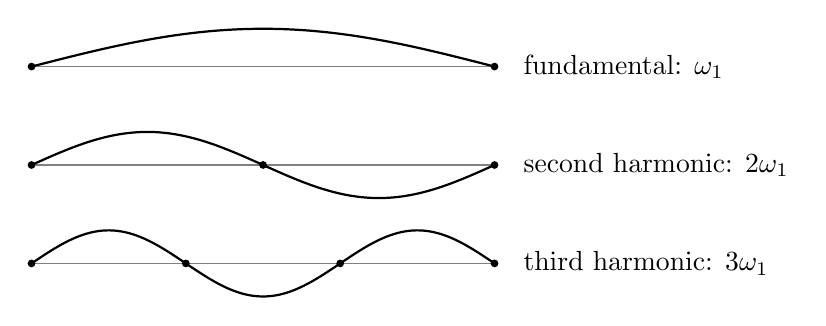
\begin{tikzpicture}[x=0.98cm,y=1cm]
\draw[gray] (0,2.5) -- (6,2.5);
\draw[thick] plot[domain=0:6,samples=120] (\x,{2.5+0.48*sin(30*\x)});
\fill (0,2.5) circle (1.4pt);
\fill (6,2.5) circle (1.4pt);
\node[right] at (6.25,2.5) {fundamental: \(\omega_1\)};

\draw[gray] (0,1.25) -- (6,1.25);
\draw[thick] plot[domain=0:6,samples=120] (\x,{1.25+0.42*sin(60*\x)});
\fill (0,1.25) circle (1.4pt);
\fill (3,1.25) circle (1.4pt);
\fill (6,1.25) circle (1.4pt);
\node[right] at (6.25,1.25) {second harmonic: \(2\omega_1\)};

\draw[gray] (0,0) -- (6,0);
\draw[thick] plot[domain=0:6,samples=120] (\x,{0.42*sin(90*\x)});
\fill (0,0) circle (1.4pt);
\fill (2,0) circle (1.4pt);
\fill (4,0) circle (1.4pt);
\fill (6,0) circle (1.4pt);
\node[right] at (6.25,0) {third harmonic: \(3\omega_1\)};
\end{tikzpicture}%
}
\caption{Le mode fondamental d’une corde et ses deuxième et troisième harmoniques, avec respectivement zéro, un et deux nœuds intérieurs.}
\end{figure}

Le mode fondamental forme un large arc et ne possède aucun nœud intérieur. C’est un oscillateur, qui peut contenir \(n_1=0,1,2,\ldots\) quanta ; chaque excitation coûte \(\hbar\omega_1\). Le deuxième harmonique possède un nœud intérieur et une fréquence double. Si le mode fondamental produit un do médian, ce mode produit le do situé une octave plus haut. Il possède un nombre d’occupation indépendant \(n_2\), et chacun de ses quanta coûte \(\hbar\omega_2=2\hbar\omega_1\). Le troisième harmonique possède deux nœuds intérieurs et une fréquence égale au triple de celle du mode fondamental. Il possède son propre nombre d’occupation indépendant \(n_3\), qui peut à nouveau être n’importe quel entier non négatif.

Mode par mode, dans la convention d’énergie utilisée plus haut, l’énergie est égale au nombre d’occupation multiplié par l’énergie du quantum. En réunissant ces contributions, on obtient
\begin{equation}
E=\sum_{N=1}^{\infty} n_N\hbar\omega_N.
\end{equation}
\editorialnote{Cette somme affichée rassemble algébriquement les énergies des modes énoncées séparément à 01:44:02--01:47:46.}

Il faut reprendre les mêmes mathématiques de l’oscillateur harmonique pour chaque mode du champ, avec un opérateur de création et un opérateur d’annihilation pour chaque oscillateur indépendant. Dans cette première représentation élémentaire, un champ quantique est l’ensemble complet de ces oscillateurs et de leur algèbre de création--annihilation.

Ce langage est adapté à la diffusion de particules. Des quanta d’énergie et de quantité de mouvement bien définies entrent dans une expérience, et d’autres quanta, d’énergies et de quantités de mouvement différentes, en sortent. Les particules incidentes sont retirées par des opérateurs d’annihilation ; les particules sortantes sont introduites dans l’état final par des opérateurs de création des modes appropriés.

\begin{classroomqa}
\lecturetimestamp{01:49:38}
\audiencequestion{Utilise-t-on le même entier pour indexer le mode de l’oscillateur et compter le nombre de quanta qu’il contient ?}
\lecturerresponse{Il s’agit de deux entiers distincts. L’indice de mode \(N\) identifie la configuration spatiale ; dans l’exemple de la corde, son nombre de nœuds détermine la fréquence \(\omega_N\). Le nombre d’occupation \(n_N\) indique combien de quanta possèdent cette fréquence.}
\end{classroomqa}